%%%%%%%%%%%%%%%%%%%%%%%%%%%%%%%%%%%%%%%%%%%%
\section{Appendix of Chapter 3}

%%%%%%%%%%%%%%%%%%%%%%%%%%%%%%%%%%%%%%%%%%%
\subsection{Proofs related to Discrete Co-Optimal Transport}

\begin{proof}[Proof of \Cref{prop:coot_gw_equiv}]
  For any $P, Q \in U(\mu_X, \mu_Y)$, we have
  \begin{align}
    \sum_{i,j,k,l} (C^x_{ik} - C^y_{jl})^2 P_{ij} Q_{kl} &=
    \mu_X^T (C^x)^{\odot 2} mu_x + \mu_Y^T (C^y)^{\odot 2}\mu_y
      - 2 \sum_{i,j,k,l} C^x_{ik} C^y_{jl} P_{ij} Q_{kl} \\
    &= \mu_X^T (C^x)^{\odot 2} mu_x + \mu_Y^T (C^y)^{\odot 2}\mu_y - 2 \tr(C^x Q C^y P^T).
  \end{align}
  Let $(P, Q)$ and $\widehat{P}$ be the solutions of the COOT and GW problems, respectively.
  As $\coot(\cX, \cY) \leq \gw(\cX, \cY)$, we have
  $\tr(C^x Q C^y P^T) \geq \tr(C^x \widehat{P} C^y \widehat{P}^T) \geq \tr(C^x Q C^y Q^T)$,
  where the second inequality is due to the suboptimality of $Q$ with respect to the GW problem.
  Given the form of $C^x$ and $C^y$, we can further simplify this inequality as
  $\tr(A Q B P^T) \geq \tr(A Q B Q^T)$. Similarly, $\tr(A Q B P^T) \geq \tr(A P B P^T)$. So,
  \begin{align} \label{eq:maron_eq}
    0 &\leq 2 \tr(AQBP^T) - \tr(AQBQ^T) - \tr(APBP^T) \\
    &= \tr \big( AQB (P-Q)^T \big) - \tr\big( A(P-Q) B P^T \big) \\
    &= \vect(Q^T) (B \otimes_K A) \vect(P-Q) - \vect(P)^T (B \otimes_K A) \vect(P-Q) \\
    &= - \vect(P-Q)^T (B \otimes_K A) \vect(P-Q),
  \end{align}
  where $\otimes_K$ denotes the Kronecker product. Now, we recall Theorem 1 in \citep{Maron18}.
  \begin{lemma} \label{lemma:maron}
    If the matrices $A \in \bbR^{m \times m}$ and $B \in \bbR^{n \times n}$
    are CND, then $\vect(X)^T (B \otimes_K A) \vect(X) \geq 0$, for every $X \in \text{lin(DS)}$,
    where $\text{lin(DS)} = \{X \in \bbR^{m \times n}: X 1_n = 0, X^T 1_m = 0 \}$.
  \end{lemma}
  As $P, Q \in U(\mu_X, \mu_Y)$, we have $P-Q \in \text{lin}(DS)$. So, by \Cref{lemma:maron},
  Inequality \eqref{eq:maron_eq} is in fact an equality, which then implies that,
  $\tr(A Q B P^T) = \tr(A Q B Q^T) = \tr(A P B P^T)$.
  We conclude that $P$ and $Q$ are two solutions of the GW problem and
  the equality between COOT and GW holds. When semi-definiteness is replaced by definiteness,
  Inequality \eqref{eq:maron_eq} becomes an equality if and only if $P=Q$.
\end{proof}

%%%%%%%%%%%%%%%%%%%%%%%%%%%%%%%%%%%%%%%%%%%%%%
\subsection{Proofs related to Continuous Co-Optimal Transport} \label{annex:cont_coot}

%%%%%%%%%%%%%%%%%%%%%%%%%%%%%%%%%%%%%%%%%
\begin{proof}[Proof of \Cref{prop:exist_coot}]
  Denote $S = X_1 \times Y_1 \times X_2 \times Y_2$.
  For convenience, we also write
  $|c_X - c_Y|^p(x_1, y_1, x_2, y_2) := |c_X(x_1, x_2) - c_Y(y_1, y_2) |^p$.
  Now, the COOT problem can be rewritten as
  \begin{equation} \label{UCOOT:1}
    \coot(\cX, \cY) = \inf_{\pi \in E_{co}} \int_{S} \vert c_X - c_Y \vert^p \; d\pi,
  \end{equation}
  where the set
  \begin{equation}
    E_{co} = \{ \pi \in \cP(S): \pi = \pi_1 \otimes \pi_2,
    \text{ where } \pi_k \in U(\mu_k^X, \mu_k^Y) \},
  \end{equation}
  contains the factorizable multi-marginal transport plans.
  Now, \Cref{lemma:compact_subset,lemma:coot_continuous}
  below imply that Problem \eqref{UCOOT:1} always admits a minimizer.
\end{proof}
%%%%%%%%%%%%%%%%%%%%%%%%%%%%%%%%%%%%%%%%%%%%%%%%
\begin{lemma} \label{lemma:product_polish}
  Countable product of Polish spaces is also a Polish space.
\end{lemma}
%%%%%%%%%%%%%%%%%%%%%%%%%%%%%%%%%%%%%%%%%
\begin{proof}[Proof of \Cref{lemma:product_polish}]
  First, the countable product of completely metrizable spaces is also completely metrizable
  (see for example, Proposition 1.4 in \citep{Dominique20})

  Second, we show that countable product of seperable spaces is also seperable.
  Given a sequence of seperable spaces $(X_k)_k$,
  let $D_k$ be a countable dense subset of $X_k$. For each $k$,
  we fix a point $x_k \in X_k$. For each integer $j \geq 1$, define
  \begin{equation}
    \widetilde{D}_j = \prod_{k=1}^j D_k \times \prod_{k > j} \{ x_k \}
    \;\; \text{ and } \;\;
    \widetilde{D} = \cup_{j} \widetilde{D}_j.
  \end{equation}
  Then clearly $\widetilde{D}_j$ is countable, for every $j \geq 1$,
  which implies $\widetilde{D}$ is also countable.
  To show that $\widetilde{D}$ is dense, every neighborhood $E$ of
  $(x_1, ..., x_k, ...)$ (after reindexing) is of the form
  $E = \prod_{k=1}^j O_k \times \prod_{k > j} \{ x_k \}$,
  for some integer $j \geq 1$ and $O_k \subset X_k$ is a neighborhood of $x_k$.
  As $D_k$ is dense in $X_k$, we have $O_k \cap D_k \neq \emptyset$,
  thus $E \cap \widetilde{D} \neq \emptyset$.
  It follows that $\widetilde{D}$ is dense in $\prod_k X_k$.
  This concludes that the countable product of Polish spaces is also a Polish space.
\end{proof}
%%%%%%%%%%%%%%%%%%%%%%%%%%%%%%%%%%%%%%%%%%%%%%%%
\begin{lemma} \label{lemma:compact_subset}
  If $X_k$ and $Y_k$ are Polish spaces, for every $k = 1, 2$,
  then $E_{co}$ is non-empty and weakly compact in $\cP(S)$.
\end{lemma}
%%%%%%%%%%%%%%%%%%%%%%%%%%%%%%%%%%%%%%%%%
\begin{proof}[Proof of \Cref{lemma:compact_subset}]
  Clearly, $(\mu_1^X \otimes \mu_1^Y) \otimes (\mu_2^X \otimes \mu_2^Y) \in E_{co}$,
  so $E_{co}$ is not empty.
  We recall that $U(\mu_1^X, \mu_1^Y, \mu_2^X, \mu_2^Y)$ is the set of admissible couplings
  whose four marginals are $\mu^X_1, \mu^Y_1, \mu^X_2$ and $\mu^Y_2$. First,
  observe that $E_{co} \subset U(\mu_1^X, \mu_1^Y, \mu_2^X, \mu_2^Y)$.
  Indeed, given $\pi_k \in U(\mu_k^X, \mu_k^Y)$, for $k = 1,2$ and denote
  $\pi = \pi_1 \otimes \pi_2 \in E_{co}$. Then, for every $i, k \in \{ 1, 2 \}$ and $i \neq k$,
  we have
  \begin{equation}
      \bigg(\int_{X_{i} \times Y_{i}} d\pi_i \bigg) \int_{Y_k}  d\pi_k = d\mu_k^X.
  \end{equation}
  Other marginal distributions can be calculated in a similar manner and we conclude that
  $\pi \in U(\mu_1^X, \mu_1^Y, \mu_2^X, \mu_2^Y)$.

  As a direct generalization of Lemma 4.4 in \citep{Villani08},
  $U(\mu_1^X, \mu_1^Y, \mu_2^X, \mu_2^Y)$ is weakly compact in $\cP(S)$. Thus,
  to show the compactness of $E_{co}$, it is enough to show that $E_{co}$
  is a weakly closed subset of $U(\mu_1^X, \mu_1^Y, \mu_2^X, \mu_2^Y)$.
  Take a sequence $(\pi^{(n)})_n \subset E_{co}$
  such that $\pi^{(n)} \rightharpoonup \pi \in U(\mu_1^X, \mu_1^Y, \mu_2^X, \mu_2^Y)$
  (due to its compactness), we need to show that $\pi \in E_{co}$.
  As $(\pi^{(n)})_n \subset E_{co}$, there exist two sequences
  $(\pi_1^{(n)})_n \subset U(\mu_1^X, \mu_1^Y)$ and $(\pi_2^{(n)})_n \subset U(\mu_2^X, \mu_2^Y)$
  such that $\pi^{(n)} = \pi_1^{(n)} \otimes \pi_2^{(n)}$.

  For each $k = 1, 2$, due to the compactness of $U(\mu_k^X, \mu_k^Y)$ in $\cP(X_k \times Y_k)$
  (Lemma 4.4 in \citep{Villani08}), we can extract a converging subsequence
  $\pi^{(n_i^{(k)})}_k \rightharpoonup \pi_k \in U(\mu_k^X, \mu_k^Y)$, when $i \to \infty$.
  By applying Theorem 2.8 in \citep{Billingsley99} on the Polish space $S$
  (thanks to \Cref{lemma:product_polish}), we have
  $\pi^{(n_i^{(1)})}_1 \otimes \pi^{(n_i^{(2)})}_2 \rightharpoonup \pi_1 \otimes \pi_2 \in E_{co}$,
  when $i \to \infty$. This implies $\pi = \pi_1 \otimes \pi_2$, thus $\pi \in E_{co}$.
\end{proof}
%%%%%%%%%%%%%%%%%%%%%%%%%%%%%%%%%
%%%%%%%%%%%%%%%%%%%%%%%%%%%%%%%%%%%%%%%%%%%%%%%%
\begin{lemma} \label{lemma:coot_continuous}
    If $c_X$ and $c_Y$ are bounded measurable functions, then
    the functional $F: \pi \to \Big( \int_{S} \vert c_X - c_Y \vert^p \; d\pi \Big)^{1/p}$ is continuous on $E_{co}$.
\end{lemma}
%%%%%%%%%%%%%%%%%%%%%%%%%%%%%%%%%%%%%%%%%
\begin{proof}[Proof of \Cref{lemma:coot_continuous}]
  It is enough to show that $F$ is continuous on $U(\mu_1^X, \mu_1^Y, \mu_2^X, \mu_2^Y)$.
  To do this, we adapt the proof of Lemma 11 in \citep{Chowdhury19} by showing that
  there exists a sequence of continuous functions converging uniformly to $F$.

  As $\cC_b$ is dense in $L^p$ (by applying Proposition 7.9 in \citep{Folland99}
  on Polish spaces endowed with finite measures), there exist two sequences of
  bounded continuous functions $(c_X^{(n)})_n \subset L^p(X, \mu^X)$ and
  $(c_Y^{(n)})_n \subset L^p(Y, \mu^Y)$ such that
  $\vert\vert c_X - c_X^{(n)} \vert\vert_{L^p(X, \mu^X)} \leq 1/n$ and
  $\vert\vert c_Y - c_Y^{(n)} \vert\vert_{L^p(Y, \mu^Y)} \leq 1/n$.

  For each $n \in \bbN$, define $F_n: U(\mu_1^X, \mu_1^Y, \mu_2^X, \mu_2^Y) \to \bbR_{\geq 0}$
  by $F_n(\pi) = \vert\vert c_X^{(n)} - c_Y^{(n)} \vert\vert_{L^p(S, \pi)}$.

  The compactness of $U(\mu_1^X, \mu_1^Y, \mu_2^X, \mu_2^Y)$ implies that, for every
  $\pi \in U(\mu_1^X, \mu_1^Y, \mu_2^X, \mu_2^Y)$,
  there exists a sequence $(\pi^{(m)})_m \subset U(\mu_1^X, \mu_1^Y, \mu_2^X, \mu_2^Y)$ such that
  $\pi^{(m)} \rightharpoonup \pi$. In particular, as
  $\vert c_X^{(n)} - c_Y^{(n)} \vert^p \in \cC_b(S)$, we have
  \begin{equation}
    \begin{split}
      \lim_{m \to \infty} F_n(\pi^{(m)}) =
      \lim_{m \to \infty} \Big( \int_{S} \vert c_X^{(n)} - c_Y^{(n)} \vert^p \;
      d\pi^{(m)} \Big)^{1/p}
      = \Big( \int_{S} \vert c_X^{(n)} - c_Y^{(n)} \vert^p \; d\pi \Big)^{1/p} = F_n(\pi).
    \end{split}
  \end{equation}
  We deduce that $F_n$ is sequentially continuous, thus continuous
  (by Remark 5.1.1 in \citep{Ambrosio05}).
  Now, for any $\pi \in U(\mu_1^X, \mu_1^Y, \mu_2^X, \mu_2^Y)$, we have
  \begin{equation}
    \begin{split}
      \vert F_n(\pi) - F(\pi) \vert &=
      \Big\vert \vert\vert c_X^{(n)} - c_Y^{(n)} \vert\vert_{L^p(S, \pi)}
      - \vert\vert c_X - c_Y \vert\vert_{L^p(S, \pi)} \Big\vert \\
      &\leq \vert\vert c_X^{(n)} - c_Y^{(n)} - (c_X - c_Y) \vert\vert_{L^p(S, \pi)} \\
      &\leq \vert\vert c_X^{(n)} - c_X \vert\vert_{L^p(S, \pi)} +
      \vert\vert c_Y^{(n)} - c_Y \vert\vert_{L^p(S, \pi)} \\
      &= \vert\vert c_X^{(n)} - c_X \vert\vert_{L^p(X, \mu^X)} +
      \vert\vert c_Y^{(n)} - c_Y \vert\vert_{L^p(Y, \mu^Y)} \\
      &\leq 2/n.
    \end{split}
  \end{equation}
  The first inequality follows from a consequence of Minkowski's inequality:
  $ \Big\vert \vert\vert f \vert\vert - \vert\vert g \vert\vert \Big\vert
  \leq \vert\vert f-g \vert\vert$. The second inequality is the Minkowski's inequality.
  This implies that $F_n$ converges uniformly to $F$, thus $F$ is continuous.
\end{proof}
%%%%%%%%%%%%%%%%%%%%%%%%%%%%%%%%%%%%%%%%%%%%%%%%

Before proving the isomorphism and metric properties of COOT, let us first introduce the Monge's
formulation of COOT.
\begin{align}
  \mcoot(\cX, \cY) =
  \inf_{\substack{T_1 \in \cT(\mu^X_1, \mu^Y_1) \\ T_2 \in \cT(\mu^X_2, \mu^Y_2)}}
  \iint \Big|c_X(x_1, x_2) - c_Y \big( T_1(x_1), T_2(x_2) \big) \Big|^p
  \; d\mu^X_1(x_1) \; d\mu^X_2(x_2),
\end{align}
where recall that
$\cT(\mu^X_k, \mu^Y_k) = \{T: X_k \to Y_k \text{ such that } T_{\#} \mu^X_k = \mu^Y_k \}$,
for $k=1,2$. It is not difficult to see that, $\mcoot(\cX, \cY) = 0$ if and only if
$\cX \in \rms(\cY)$. Similar to the GW and Gromov-Monge distances, we have
%%%%%%%%%%%%%%%%%%%%%%%%%%%%%%%
\begin{corollary} \label{coro:coot_mcoot}
  Let $\cX$ and $\cY$ be two measure hypernetworks, then
  \begin{equation}
    \coot(\cX, \cY) = \inf_{\cZ \in \rms(\cX)} \mcoot(\cZ, \cY)
    = \inf_{\cZ \in \rms(\cY)} \mcoot(\cZ, \cX).
  \end{equation}
  Moreover, the infima are always attained: there exist two measure hypernetworks
  $\cZ_x \in \rms(\cX)$ and $\cZ_y \in \rms(\cY)$ such that
  $\coot(\cX, \cY) = \mcoot(\cZ_x, \cY) = \mcoot(\cZ_y, \cX)$.
\end{corollary}
The proof is adapted directly from that of Theorem 14 in \citep{Memoli21}.
For self-contained purpose, we provide the complete proof here.
%%%%%%%%%%%%%%%%%%%%%%%%%%%%%%%%%%%%%%%%%
\begin{proof}[Proof of \Cref{coro:coot_mcoot}]
  Let $(\pi_1^*, \pi_2^*)$ be a solution of the problem $\coot(\cX, \cY)$.
  For $k=1,2$, define the space $Z_k = X_k \times Y_k$
  equipped with the probability measure $\mu_k^Z = \pi_k^* \in U(\mu_k^X, \mu_k^Y)$.
  Define the projection map $P_{X_k}: Z_k \to X_k$ by $P_{X_k}(x,y) = x$ and denote
  $c_Z = (P_{X_1}, P_{X_2})^*c_X$. Clearly, the measure hypernetwork
  $\cZ := ((Z_1, \mu_1^Z), (Z_2, \mu_2^Z), c_Z)$ is a RMS of $\cX$. For
  $k=1,2$, consider the canonical projection map $P_{Y_k}: Z_k \to Y_k$ defined by $P_{Y_k}(x,y) = y$,
  then $P_{Y_k}$ is a transport map from $\mu_k^Z$ to $\mu_k^Y$. Now, as
  $(P_{X_k}, P_{Y_k})_{\#} \mu_k^Z = (P_{X_k}, P_{Y_k})_{\#} \pi_k^* = \pi_k^*$,
  for $k=1,2$, we have
  \begin{align}
    \mcoot(\cZ, \cY) &\leq \int_{Z_1 \times Z_2}
    \big\vert c_Z - (P_{Y_1}, P_{Y_2})^*c_Y \big\vert^p \; d\mu_1^Z \; d\mu_2^Z \\
    &= \int_{Z_1 \times Z_2}
    \big\vert (P_{X_1}, P_{X_2})^*c_X - (P_{Y_1}, P_{Y_2})^*c_Y \big\vert^p
    \; d\mu_1^Z \; d\mu_2^Z \\
    &= \int_{S} \vert c_X - c_Y \vert^p
    \; d(P_{X_1}, P_{Y_1})_{\#} \mu_1^Z \; d(P_{X_2}, P_{Y_2})_{\#} \mu_2^Z \\
    &= \int_{S} \vert c_X - c_Y \vert^p \; d\pi_1^* \; d\pi_2^* \\
    &= \coot(\cX, \cY),
  \end{align}
  and consequently,
  \begin{equation}
    \label{eq:coot_geq_mcoot}
    \coot(\cX, \cY) \geq \inf_{\cZ \in \rms(\cX)} \mcoot(\cZ, \cY).
  \end{equation}
  For the reverse direction, let $\cZ$ be a RMS of $\cX$. Then,
  there exist two transport maps $f_k : Z_k \to X_k$, for $k=1,2$ such that $c_Z = (f_1, f_2)^*c_X$,
  for $\mu_1^Z \otimes \mu_2^Z$-almost everywhere.
  The inequality \eqref{eq:coot_geq_mcoot} implies that we can safely exclude every
  $\cZ \in \rms(\cX)$ with $\mcoot(\cZ, \cY) = \infty$ and consider only those with
  $\mcoot(\cZ, \cY) < \infty$. In this case, there always exists a transport map
  $g_k$ from $\mu_k^Z$ to $\mu_k^Y$, for each $k=1,2$. If we define the map
  $(f_k, g_k): Z_k \to X_k \times Y_k$ by $(f_k,g_k)(z_k) = (f_k(z_k), g_k(z_k))$,
  then $(f_k,g_k)_{\# \mu_k^Z} \in U(\mu_k^X, \mu_k^Y)$, for any $k=1,2$. Now,
  \begin{align}
    \coot(\cX, \cY) &\leq \int_{S} \vert c_X - c_Y \vert^p
    \; d (f_1,g_1)_{\#} \mu_1^Z \; d (f_2,g_2)_{\#} \mu_2^Z \\
    &= \int_{Z_1 \times Z_2} \vert (f_1,f_2)^*c_X - (g_1,g_2)^*c_Y \vert^p \; d\mu_1^Z \; d\mu_2^Z \\
    &= \int_{Z_1 \times Z_2} \vert c_Z - (g_1,g_2)^*c_Y \vert^p \; d\mu_1^Z \; d\mu_2^Z.
  \end{align}
  As this is true for any $\cZ \in \rms(\cX)$ and any corresponding pair of transport maps
  $(g_1, g_2)$, we have
  \begin{equation}
    \coot(\cX, \cY) \leq \inf_{\cZ \in \rms(\cX)} \mcoot(\cZ, \cY).
  \end{equation}
  The equality then follows. Moreover, the first part of the proof also
  shows us how to construct a minimizer $\cZ_x \in \rms(\cX)$ such that
  $\coot(\cX, \cY) = \mcoot(\cZ_x, \cY)$. Similarly, we have
  \begin{equation}
    \coot(\cY, \cX) = \inf_{\cZ \in \rms(\cY)} \mcoot(\cZ, \cX).
  \end{equation}
  By the symmetry of COOT, we deduce that
  \begin{equation}
    \inf_{\cZ \in \rms(\cX)} \mcoot(\cZ, \cY) = \inf_{\cZ \in \rms(\cY)} \mcoot(\cZ, \cX),
  \end{equation}
  and there exists $\cZ_y \in \rms(\cY)$ such that $\coot(\cX, \cY) = \mcoot(\cZ_y, \cX)$.
\end{proof}
%%%%%%%%%%%%%%%%%%%%%%%%%%%%%%%%%%%%%%%%%%%%%%%%

%%%%%%%%%%%%%%%%%%%%%%%%%%%%%%%%%%%%%%%%%%%%%
\begin{proof}[Proof of \Cref{prop:strong_weak_iso}]
Let us first prove the following simple lemma.
\begin{lemma} \label{lemma:bijection}
  Let $f: X \to Y$ be a surjective map. If $X$ and $Y$ are finite and have the same cardinal,
  then $f$ is bijective.
\end{lemma}
\begin{proof}
  Suppose $| X | = | Y | = n$. As $f$ is surjective, for each $y \in Y$,
  the set $X(y) := \{ x \in X: f(x) = y \}$ is not empty, \ie, $| X(y) | \geq 1$.
  Clearly, $\cup_y X(y) \subset X$ and $X(y) \cap X(y') = \emptyset$, for any $y \neq y'$.
  Thus $| X | \geq | \cup_y X(y) | = \sum_y |X(y)| \geq n$.
  We deduce that $|X(y)| = 1$, for every $y \in Y$, thus $f$ is bijective.
\end{proof}
Now,
\begin{enumerate}
  \item Clearly, strong isomorphism implies semi-strong isomorphism.
  Suppose $\cX$ and $\cY$ are semi-strongly isomorphic, then $\cX$ is a common RMS of
  $\cX$ and $\cY$, meaning that $\cX$ and $\cY$ are weakly isomorphic.

  \item Let $\cX$ and $\cY$ be two finite measure hypernetworks.
  Suppose semi-strong isomorphism holds, then there exist four transport maps
  $f_k: X_k \to Y_k$ and $g_k: Y_k \to X_k$ such that $(f_k)_{\#} \mu_k^X = \mu_k^Y$ and
  $(g_k)_{\#} \mu_k^Y = \mu_k^X$, for $k=1,2$, and two pullback equalities hold everywhere.
  As a transport map is necessarily surjective, we must have $| Y_k | \geq | X_k|$
  and $| X_k | \geq | Y_k|$, thus $| Y_k | = | X_k|$. By \Cref{lemma:bijection},
  we deduce that $f_k$ (and $g_k$) are bijective. The strong isomorphism then follows.

  \item By \Cref{prop:coot_iso}, the weak isomorphism implies $\coot(\cX, \cY) = 0$.
  By Proposition 1 in \citep{Redko20}, there exist two permutations (thus Borel measurable bijections)
  $\sigma_k: X_k \to Y_k$, for $k=1,2$, such that $c_X(i_1,i_2) = c_Y(\sigma_1(i_1), \sigma_2(i_2))$,
  for every $(i_1,i_2) \in X_1 \times X_2$. Furthermore, for every $j \in Y_k$,
  there exists a unique $i \in X_k$ such that $j = \sigma_k(i)$. Thus, by hypothesis, we have
  \begin{equation}
    \mu_k^Y(j) = \frac{1}{\vert Y_k \vert} = \frac{1}{\vert X_k \vert} =
    \mu_k^X(i) = \sum_{i': \sigma_k(i') = j} \mu_k^X(i'),
  \end{equation}
  which means $(\sigma_k)_{\#} \mu_k^X = \mu_k^Y$. So $\cX$ is a RMS of $\cY$. Similarly,
  $\cY$ is also a RMS of $\cX$. The semi-strong isomorphism then follows.
\end{enumerate}
\end{proof}

%%%%%%%%%%%%%%%%%%%%%%%%%%%%%%%%%%%%%%%%%%%%%%%%
\begin{proof}[Proof of \Cref{prop:coot_iso}]
    Suppose two measure hypernetworks $\cX$ and $\cY$ are weakly isomorphic,
    then there exists a measure hypernetwork $\cZ^*$ which is a common RMS of $\cX$ and $\cY$.
    In particular, $\mcoot(\cZ^*, \cY) = 0$. By \Cref{coro:coot_mcoot}, we deduce that
    \begin{equation}
      \coot(\cX, \cY) = \inf_{\cZ \in \rms(\cX)} \mcoot(\cZ, \cY) = 0.
    \end{equation}
    Now, suppose $\coot(\cX, \cY)=0$, then by \Cref{coro:coot_mcoot},
    there exists $\cZ^* \in \rms(\cX)$ such that $\mcoot(\cZ^*, \cY) = 0$.
    But this also means $\cZ^*$ is a RMS of $\cY$.
    We conclude that $\cX$ and $\cY$ are weakly isomorphic.
\end{proof}
%%%%%%%%%%%%%%%%%%%%%%%%%%%%%%%

%%%%%%%%%%%%%%%%%%%%%%%%%%%%%%%
\begin{proof}[Proof of \Cref{prop:metric_prop}]
  The proof of this result can be found in \citep{Chowdhury21b}.
  However, we still provide our proof here (slightly different but based on the same techniques).

  For clarity, given three measure hypernetworks $\cX, \cY$ and $\cZ$,
  we denote $S_{xy} = \prod_{k=1}^2 X_k \times Y_k, S_{yz} = \prod_{k=1}^2 Y_k \times Z_k,
  S_{xz} = \prod_{k=1}^2 X_k \times Z_k$ and $S_{xyz} = \prod_{k=1}^2 X_k \times Y_k \times Z_k$.
  \begin{enumerate}
    \item The positiveness is trivial. By \Cref{prop:coot_iso},
    $\coot(\cX, \cY) = 0$ if and only if $\cX$ and $\cY$ are weakly isomorphic.

    \item To show the symmetry, for each $k = 1, 2$, we define the bijection
    $f_k: X_k \times Y_k \to Y_k \times X_k$ by $f_k(x_k,y_k) = (y_k,x_k)$.
    Then, for any $\pi_k \in U(\mu_k^X, \mu_k^Y)$, where $k=1,2$, we have
    $(f_k)_{\#} \pi_k \in U(\mu_k^Y, \mu_k^X)$ and
    \begin{equation}
      \begin{split}
        \coot(\cX, \cY) &= \inf_{\substack{\pi_k \in U(\mu^X_k, \mu^Y_k) \\
        \forall k = 1,2}} \int_{S_{xy}} \vert c_X - c_Y \vert^p \; d \pi_1 \; d \pi_2 \\
        &= \inf_{\substack{\pi_k \in U(\mu^X_k, \mu^Y_k) \\
        \forall k = 1,2}} \int_{S_{yx}} \vert c_Y - c_X \vert^p \; d (f_1)_{\#} \pi_1 \; d (f_2)_{\#} \pi_2 \\
        &= \inf_{\substack{\gamma_k \in U(\mu^Y_k, \mu^X_k) \\
        \forall k = 1,2}} \int_{S_{yx}} \vert c_Y - c_X \vert^p \; d \gamma_1 \; d \gamma_2 \\
        &= \coot(\cY, \cX).
      \end{split}
    \end{equation}

    \item Now, we show the triangle inequality. Let $(\pi^{(YZ)}_1, \pi^{(YZ)}_2)$ and
    $(\pi^{(XZ)}_1, \pi^{(XZ)}_2)$ be the optimal couplings which minimize
    $\coot(\cY, \cZ)$ and $\coot(\cX, \cZ)$, respectively, where
    $\pi^{(YZ)}_k$ and $\pi^{(XZ)}_k$ are in $U(\mu_k^Y, \mu_k^Z)$ and $U(\mu_k^X, \mu_k^Z)$,
    respectively, for every $k=1,2$.

    For each $k = 1,2$, by the glueing lemma (Lemma 7.6 in \citep{Villani03}), there exists a probability measure
    $\sigma_k \in \cP(X_k \times Y_k \times Z_k)$ such that
    $(P_{X_k Y_k})_{\#} \sigma_k = \pi^{(XY)}_k$ and
    $(P_{X_k Y_k})_{\#} \sigma_k = \pi^{(YZ)}_k$. Here, we define the projection maps
    \begin{itemize}
      \item[$\bullet$] $P_{X_k}: X_k \times Y_k \times Z_k \to X_k$, where
      $P_{X_k}(x,y,z) = x$.
      \item[$\bullet$] $P_{X_k Y_k}: X_k \times Y_k \times Z_k \to X_k \times Y_k$,
      where $P_{X_k Y_k}(x,y,z) = (x,y)$.
      \item[$\bullet$] $P_{X_1 Z_1 X_2 Z_2}: S_{xyz} \to S_{xz}$, where
      $P_{X_1 Z_1 X_2 Z_2}(x_1,y_1,z_1, x_2, y_2, z_2) = (x_1,z_1, x_2, z_2)$.
    \end{itemize}
    and all other projection maps are defined similarly. It follows that
    $(P_{X_k})_{\#} \sigma_k = \mu_k^X$ and $(P_{Z_k})_{\#} \sigma_k = \mu_k^Z$, thus
    $(P_{X_k Z_k})_{\#} \sigma_k \in U(\mu_k^X, \mu_k^Z)$. Furthermore, one also has
    $(P_{X_1 Z_1 X_2 Z_2})_{\#} \sigma =
    (P_{X_1 Z_1})_{\#} \sigma_1 \otimes (P_{X_2 Z_2})_{\#} \sigma_2$,
    where $\sigma = \sigma_1 \otimes \sigma_2$. Indeed, for any function $\phi \in \cC_b(S_{xz})$, we have
    \begin{equation}
      \begin{split}
        \int_{S_{xz}} \phi \; d(P_{X_1 Z_1 X_2 Z_2})_{\#} \sigma
        &= \int_{S_{xyz}} (\phi \circ P_{X_1 Z_1 X_2 Z_2}) \; d\sigma \\
        &= \int_{S_{xyz}} (P_{X_1 Z_1}, P_{X_2 Z_2})^*\phi
        \; d \sigma_1 \; d \sigma_2 \\
        &= \int_{S_{xz}} \phi \; d (P_{X_1 Z_1})_{\#} \sigma_1 \;
        d (P_{X_2 Z_2})_{\#} \sigma_2.
      \end{split}
    \end{equation}
    Here, with slight abuse of notation, we write $\phi(x_1,y_1, x_2,y_2) = \phi\big( (x_1,y_1), (x_2,y_2) \big)$. Now,
    \begin{equation}
      \begin{split}
        &\coot(\cX, \cZ)^{1/p} \\
        &\leq \Big( \int_{S_{xz}} \vert c_X - c_Z \vert^p
        \; d (P_{X_1 Z_1})_{\#} \sigma_1 \; d (P_{X_2 Z_2})_{\#} \sigma_2 \Big)^{1/p} \\
        &= \Big( \int_{S_{xz}} \vert c_X - c_Z \vert^p
        \; d(P_{X_1 Z_1 X_2 Z_2})_{\#} \sigma \Big)^{1/p} \\
        &= \Big( \int_{S_{xyz}} \big( \vert c_X - c_Z \vert^p \circ P_{X_1 Z_1 X_2 Z_2} \big)
        \; d \sigma \Big)^{1/p} \\
        &\leq \Big( \int_{S_{xyz}} \big( \vert c_X - c_Y \vert^p \circ P_{X_1 Y_1 X_2 Y_2} \big)
        \; d \sigma \Big)^{1/p} +
        \Big( \int_{S_{xyz}} \big( \vert c_Y - c_Z \vert^p \circ P_{Y_1 Z_1 Y_2 Z_2} \big)
        \; d \sigma \Big)^{1/p} \\
        &= \Big( \int_{S_{xy}} \vert c_X - c_Y \vert^p
        \; d (P_{X_1 Y_1 X_2 Y_2})_{\#} \sigma \Big)^{1/p}  +
        \Big( \int_{S_{yz}} \vert c_Y - c_Z \vert^p
        \; d (P_{Y_1 Z_1 Y_2 Z_2})_{\#} \sigma \Big)^{1/p}  \\
        &= \Big( \int_{S_{xy}} \vert c_X - c_Y \vert^p
        \; d (P_{X_1 Y_1})_{\#} \sigma_1 \; d (P_{X_2 Y_2})_{\#} \sigma_2 \Big)^{1/p} \\
        &+ \Big( \int_{S_{yz}} \vert c_Y - c_Z \vert^p
        \; d (P_{Y_1 Z_1})_{\#} \sigma_1 \; d (P_{Y_2 Z_2})_{\#} \sigma_2 \Big)^{1/p} \\
        &= \Big( \int_{S_{xy}} \vert c_X - c_Y \vert^p \; d \pi^{(XY)}_1 \; d \pi^{(XY)}_2 \Big)^{1/p}  +
        \Big( \int_{S_{yz}} \vert c_Y - c_Z \vert^p \; d \pi^{(YZ)}_1 \; d \pi^{(YZ)}_2 \Big)^{1/p} \\
        &= \coot(\cX, \cY)^{1/p} + \coot(\cY, \cZ)^{1/p}.
      \end{split}
    \end{equation}
    The first inequality is due to the sub-optimality of
    $((P_{X_1 Z_1})_{\#} \sigma_1, (P_{X_2 Z_2})_{\#} \sigma_2)$. The second one is
    the Minkowski inequality and the fact that:
    $|c_X(x_1,x_2) - c_Y(y_1,y_2)| \leq |c_X(x_1,x_2) - c_Z(z_1,z_2)| + |c_Z(z_1,z_2) - c_Y(y_1,y_2)|$,
    or more compactly
    \begin{equation}
      \vert c_X - c_Z \vert \circ P_{X_1 Z_1 X_2 Z_2} \leq
      \vert c_X - c_Y \vert \circ P_{X_1 Y_1 X_2 Y_2} +
      \vert c_Y - c_Z \vert \circ P_{Y_1 Z_1 Y_2 Z_2}.
    \end{equation}
  \end{enumerate}
\end{proof}
%%%%%%%%%%%%%%%%%%%%%%%%%%%%%%%%%

%%%%%%%%%%%%%%%%%%%%%%%%%%%%%%
% \begin{proof}[Proof of \Cref{prop:conv_ent_coot}]

%     %%%%%%%%%%%%%%%%%%%%%%%%%%%%%%%%%%%%%%%%%%%%%
%     \begin{lemma}
%         \label{lemma:block_approx}
%       Recall that $U(\mu_1, ..., \mu_K)$ is the set of couplings whose marginals are $\mu_1,...,\mu_K$.
%       For each $\pi \in U(\mu_1, ..., \mu_K)$, denote $\pi_{\Delta}$ its block approximation at scale $\Delta > 0$.
%       \begin{enumerate}
%         \item The entropy $H(\pi)$ is well defined and
%         \begin{equation}
%           \kl(\pi \vert \otimes_k \mu_k) = H(\pi) - \sum_{k=1}^K H(\mu_k).
%         \end{equation}

%         \item For every $\Delta > 0, \pi_{\Delta} \in U(\mu_1, ..., \mu_K)$.

%         \item Suppose the product space $\prod_k \bbR^{n_k}$ is endowed with the metric
%         \begin{equation}
%           d((x_1, ..., x_K), (y_1, ..., y_K)) = \Big( \sum_{k=1}^K \vert\vert x_k - y_k \vert\vert^p \Big)^{1/p}.
%         \end{equation}
%         Then
%         \begin{equation}
%           W^p_{d^p}(\pi, \pi_{\Delta}) \leq \Big( \sum_{k=1}^K n_k \Big) \Delta^p,
%         \end{equation}
%         where $W_{d^p}(\pi, \pi_{\Delta})$ is the $p$-Wasserstein distance between $\pi$ and $\pi_{\Delta}$ induced by the cost $d^p$.
%         Consequently, $\pi_{\Delta} \rightharpoonup \pi$ when $\Delta \to 0$.

%         \item There exists constants $C > 0$ and $\alpha \in (0,1)$ such that
%         \begin{equation}
%           \kl(\pi_{\Delta} \vert \otimes_k \mu_k) \leq
%           \sum_{k=1}^K \Big( C \big( M(\mu_k) + n_k \Delta^2 + 1 \big)^{\alpha} - n_k \log \Delta \Big).
%         \end{equation}
%       \end{enumerate}
%     \end{lemma}
%     %%%%%%%%%%%%%%%%%%%%%%%%%%%%%%%%%%%%%%%%%
%     \begin{proof}
%       Most proofs follow directly from \citep{Carlier17}.
%       \begin{enumerate}
%         \item If $\pi \ll \otimes_k \mu_k$, then as $\mu_k \ll \lambda_k$, we must have $\pi \ll \otimes_k \lambda_k$. Thus $H(\pi)$ is well
%         defined. Furthermore,
%         \begin{equation}
%           \begin{split}
%             \kl(\pi \vert \otimes_k \mu_k)
%             &= \int \log \Big( \frac{\pi(x_1,...,x_K)}{\mu_1(x_1)...\mu_K(x_K)} \Big) \pi(x_1, ..., x_K) \; dx_1 ... dx_K \\
%             &= \int \pi \log \pi - \sum_{k=1}^K \int \pi(x_1, ..., x_K) \log \mu_k(x_k) \; dx_1 ... dx_K \\
%             &= H(\pi) - \sum_{k=1}^K \int \pi_{\# k}(x_k) \log \mu_k(x_k) \; dx_k \\
%             &= H(\pi) - \sum_{k=1}^K \int \mu_k(x_k) \log \mu_k(x_k) \; dx_k \\
%             &= H(\pi) - \sum_{k=1}^K H(\mu_k).
%           \end{split}
%         \end{equation}

%         \item See Proposition 2.10 in \citep{Carlier17}
%         \item See Lemma 2.11 and corollary 2.12 in \citep{Carlier17}
%         \item See Proposition 2.14 in \citep{Carlier17}.
%       \end{enumerate}
%     \end{proof}
%     %%%%%%%%%%%%%%%%%%%%%%%%%%%%%%%%%%%%%%%%%%%%%
%     \begin{lemma} \label{lemma:limsupinf}
%       Under Assumption 2a in the Proposition ,
%       let $E$ be a non-empty subset of $\cP(S)$ and $(\varepsilon_n)_n$ be a positive sequence converging to zero.
%       Define $\widetilde{F}: \cP(S) \to \bbR \cup \{ \infty \}$ and
%       $\widetilde{F}_n: \cP(S) \to \bbR \cup \{ \infty \}$ by
%       \begin{equation}
%         \widetilde{F}(\pi) =
%         \begin{cases}
%           \int_{S} \vert c_X - c_Y \vert^p \; d\pi, \text{ if } \pi \in E \\
%           \infty \;\;\;\;\;\;\;\;\;\;\;\;\;\;\;\;\;\;\;\;\; ,\text{ otherwise},
%         \end{cases}
%       \end{equation}
%       and
%       \begin{equation}
%         \widetilde{F}_n(\pi) =
%         \begin{cases}
%           \int_{S} \vert c_X - c_Y \vert^p \; d\pi + \varepsilon_n \kl(\pi \vert \mu_1 \otimes \mu_2), \text{ if } \pi \in E \\
%           \infty \;\;\;\;\;\;\;\;\;\;\;\;\;\;\;\;\;\;\;\;\;\;\;\;\;\;\;\;\;\;\;\;\;\;\;\;\;\;\;\;\;\;\;\;\;\;\;\;\;\;\;\; ,\text{ otherwise}.
%         \end{cases}
%       \end{equation}
%       \begin{enumerate}
%         \item Assume that if $\pi \in E$, then so is its block approximation. Then for every $\pi \in E$ and positive sequence $(\Delta_n)_n \to 0$, we have
%         \begin{equation}
%           \widetilde{F}(\pi) \geq \lim\sup_{n \to \infty} \widetilde{F}_{\Delta_n}(\pi_{\Delta_n}).
%         \end{equation}

%         \item Let $(\pi_n)_n \subset \cP(S)$ be a sequence weakly converging to $\pi \in E$. Then
%         \begin{equation}
%           F(\pi) \leq \lim \inf_{n \to \infty} F_{n}(\pi_n).
%         \end{equation}
%       \end{enumerate}
%     \end{lemma}
%     %%%%%%%%%%%%%%%%%%%%%%%%%%%%%%%%%%%%%%%%%
%     \begin{proof}[Proof of \Cref{lemma:limsupinf}]
%       \text{ }
%       \begin{enumerate}
%         \item When $S$ is a finite-dimensional vector space, by \Cref{lemma:block_approx} and
%         definition 6.8 in \citep{Villani08}, when $n \to \infty$,
%         \begin{equation}
%           \int_S \vert c_X - c_Y\vert^p \; d\pi_{\Delta_n} \to \int_S \vert c_X - c_Y\vert^p \; d\pi.
%         \end{equation}
%         On the other hand, following \Cref{lemma:block_approx} and the proof of the proposition 2.16 in \citep{Carlier17}, we have
%         \begin{equation}
%           \lim\sup_{n \to \infty} \Delta_n \kl(\pi_{\Delta_n} \vert \mu_1 \otimes \mu_2) \leq 0.
%         \end{equation}
%         The claim then follows.

%         \item This is true because the KL divergence is nonnegative and the other terms are lower semicontinuous.
%       \end{enumerate}
%     \end{proof}
%     %%%%%%%%%%%%%%%%%%%%%%%%%%%%%%%%%%%%%%%%%%%%%
%     Now, we complete the proof of the .
%     When $\varepsilon \to 0$, in case of finite-dimensional spaces, if $\pi \in E_{co}$ (or $E_{gw}$), then so is its block approximation.
%     We deduce from \Cref{lemma:limsupinf} that $\widetilde{F}_{n}$ $\Gamma$-converges to
%     $\widetilde{F}$, whenever $E = E_{co}$ or $E = E_{gw}$. Moreover, in both cases, the weak compactness of $E$ implies the equi-coercivity
%     of $\widetilde{F}_n$. By the theorems 7.8 and 7.18 in \citep{Maso93}, we deduce that
%     $\coot_{\varepsilon_n}(\cX, \cY) \to \coot(\cX, \cY)$, when $\varepsilon_n \to 0$,
%     and if $(\pi_{\varepsilon_n})_{n}$ is a sequence of solution of $\coot_{\varepsilon_n}(\cX, \cY)$,
%     then any cluster point of $(\pi_{\varepsilon_n})_{n}$ is a solution of $\coot(\cX, \cY)$.
%   \end{proof}
% %%%%%%%%%%%%%%%%%%%%%%%%%%%%%%%

%%%%%%%%%%%%%%%%%%%%%%%%%%%%%%%
Recall that
\begin{equation}
  E_{co} = \{ \pi \in \cP(S): \pi = \pi_1 \otimes \pi_2,
  \text{ where } \pi_k \in U(\mu_k^X, \mu_k^Y) \}.
\end{equation}
First, observe that if $\pi \in E_{co}$ is a solution of COOT, then for any $\gamma \in E_{co}$, one has
\begin{equation}
  \begin{split}
    0 &\leq \coot_{\varepsilon}(\cX, \cY) - \coot(\cX, \cY) \\
    &\leq \left( \int_{S} \vert c_X - c_Y \vert^p \; d\gamma - \int_{S} \vert c_X - c_Y \vert^p \; d\pi \right) +
    \varepsilon \kl(\gamma \vert \mu_1 \otimes \mu_2).
  \end{split}
\end{equation}
The idea is to choose $\gamma \in E_{co}$ such that, for small $\varepsilon$, the quantity inside the bracket can be arbitrarily small
(but still positive, due to the optimality of $\pi$), and the KL divergence is always controlled, so that it does not blow up too fast.
To do so, we extend the block approximation technique \citep{Carlier17} to the multi-marginal case.
\begin{definition}
  (Block approximation) Given an integer $K \geq 2$ and $p \geq 1$. For each $k=1,...,K$,
  let $\mu_k \in \cP(\bbR^{n_k})$, for some integer $n_k \geq 1$, be a probability measure.
  % with finite entropy and $p^{\text{th}}$-moment and
  % absolutely continuous with respect to the Lebesgue measure.
  For each tuple of integers $a_k = (a_k^{(1)}, ...,a_k^{(n_k)}) \in \bbZ^{n_k}$, we define the unit hypercube
  $Q_{a_k} = [a_k^{(1)}, a_k^{(1)} + 1[ \times ... \times [a_k^{(n_k)}, a_k^{(n_k)} + 1[ \subset \bbR^{n_k}$ and for $\Delta > 0$,
  we denote $Q^{\Delta}_{a_k} = [\Delta a_k^{(1)}, \Delta(a_k^{(1)} + 1)[ \times ... \times [\Delta a_k^{(n_k)}, \Delta(a_k^{(n_k)} + 1)[ \subset \bbR^{n_k}$ the rescaled hypercube by $\Delta$ of $Q_{a_k}$.
  For each $\pi \in \cP(\prod_k \bbR^{n_k})$, we define its block approximation at scale $\Delta$ by
  \begin{equation}
    \pi_{\Delta} := \sum_{\substack{a_k \in \bbZ^{n_k} \\ k = 1, ..., K}}
    \pi \big(\prod_{k=1}^K Q^{\Delta}_{a_k}\big) \big( \otimes_{k=1}^K \mu_k^{\Delta} \big),
  \end{equation}
  where, for every Borel set $E_k \subset \bbR^{n_k}, \mu_k^{\Delta}$ is the restriction of $\mu_k$ on $Q^{\Delta}_{a_k}$ defined by
  \begin{equation}
    \mu_k^{\Delta}(E_k):=
    \begin{cases}
      \frac{\mu_k(E_k \cap Q^{\Delta}_{a_k})}{\mu_k(Q^{\Delta}_{a_k})} \; ,\text{ if } \mu_k(Q^{\Delta}_{a_k}) > 0 \\
      0 \;\;\;\;\;\;\;\;\;\;\;\;\;\;\;\;,\text{ otherwise}.
    \end{cases}
  \end{equation}
\end{definition}
It is not difficult to see that block approximation of a product measure is also a product measure. Indeed, it is enough to consider the case
$K=2$. Suppose that $\pi = \pi_1 \otimes \pi_2$, then for any $\Delta > 0$,
\begin{equation}
  \pi_{\Delta} = \sum_{a_1, a_2}
  \pi_1(Q^{\Delta}_{a_1}) \; \pi_2(Q^{\Delta}_{a_2}) \; \mu_1^{\Delta} \otimes \mu_2^{\Delta} =
  \left( \sum_{a_1} \pi_1(Q^{\Delta}_{a_1}) \; \mu_1^{\Delta} \right) \otimes
  \left( \sum_{a_2} \pi_2(Q^{\Delta}_{a_2}) \; \mu_2^{\Delta} \right).
\end{equation}
Also, if a coupling is admissible, then so is its block approximation. More precisely,
by Proposition 2.10 in \citep{Carlier17}, for any $\pi \in U(\mu_1, ..., \mu_K)$ and $\Delta > 0$,
we have $\pi_{\Delta} \in U(\mu_1, ..., \mu_K)$.

\begin{proof}[Proof of \Cref{prop:quant_bound_ent}]
  This is an adaptation from the proof of quantitative bound between OT and regularized OT
  in \citep{Genevay19}.
  Let $\pi^* \in E_{co}$ be a solution of COOT and denote $\pi_{\Delta}$
  its block approximation at scale $\Delta > 0$.
  Clearly, $\pi_{\Delta} \in E_{co}$. Denote $\mu = \mu_X \otimes \mu_Y$.
  The sub-optimality of $\pi_{\Delta}$ implies
  \begin{align}
      0 &\leq \coot_{\varepsilon}(\cX, \cY) - \coot(\cX, \cY) \\
      &\leq \langle \pi_{\Delta}, \vert c_X - c_Y \vert^p \rangle
      - \langle \pi^*, \vert c_X - c_Y \vert^p \rangle +
      \varepsilon \kl(\pi_{\Delta} \vert \mu \otimes \mu).
  \end{align}
  Now, using the fact that $\vert x - y \vert \leq \max(x,y)$, for every $x, y \geq 0$,
  and for any $i,j$,
  \begin{equation}
    \sup_{(x_1, x_2) \in Q^{\Delta}_{ij}} |c_X(x_1,x_2)|
    \leq L \sup_{(x_1, x_2) \in Q^{\Delta}_{ij}} \vert\vert x_1 - x_2 \vert\vert^q
    \leq L (\Delta d_x^{1/p})^q,
  \end{equation}
  we deduce that
  \begin{align}
    \langle \pi_{\Delta}, \vert c_X - c_Y \vert^p \rangle
    - \langle \pi^*, \vert c_X - c_Y \vert^p \rangle
    &\leq \sup_{i,j,k,l} \sup_{\substack{(x_1, x_2) \in Q^{\Delta}_{ij} \\
    (y_1,y_2) \in Q^{\Delta}_{kl}}} \vert c_X(x_1,x_2) - c_Y(y_1,y_2) \vert^p \\
    &\leq \max \big\{ \sup_{(x_1, x_2) \in Q^{\Delta}_{ij}} |c_X(x_1,x_2)|^p,
    \sup_{(y_1, y_2) \in Q^{\Delta}_{kl}} |c_Y(y_1,y_2)|^p \big\} \\
    &\leq \max \big\{ L^p (\Delta d_x^{1/p})^{pq}, L^p (\Delta d_y^{1/p})^{pq} \big\} \\
    &= L^p \Delta^{pq} d^q.
  \end{align}
  Following the proof of Theorem 1 in \citep{Genevay19}, we obtain the bound for the KL term
  \begin{equation}
      \kl(\pi^{\Delta} | \mu \otimes \mu)
      \leq 2(d_x + d_y) \log(\frac{2D}{\Delta}) \leq 4 d \log(\frac{2D}{\Delta}).
  \end{equation}
  So, we have
  \begin{equation}
    \langle \pi_{\Delta}, \vert c_X - c_Y \vert^p \rangle -
    \langle \pi^*, \vert c_X - c_Y \vert^p \rangle + \varepsilon \kl(\pi^{\Delta} | \mu \otimes \mu)
    \leq L^p \Delta^{pq} d^q + 4 d \varepsilon \log(\frac{2D}{\Delta}).
  \end{equation}
  The RHS is a convex function of $\Delta$, thus admits a minimizer
  $\Delta^{pq} = \frac{4d \varepsilon}{L^p d^q pq}$, thus
  \begin{equation}
    \langle \pi_{\Delta}, \vert c_X - c_Y \vert^p \rangle
    - \langle \pi^*, \vert c_X - c_Y \vert^p \rangle + \varepsilon \kl(\pi^{\Delta} | \mu \otimes \mu)
    \leq \frac{4 d \varepsilon}{pq}
    + \frac{4d \varepsilon}{pq} \log\Big( \frac{(2D)^{pq} L^p d^q pq}{4d \varepsilon} \Big).
  \end{equation}
  The result then follows.
\end{proof}
%%%%%%%%%%%%%%%%%%%%%%%%%%%%%%%

%%%%%%%%%%%%%%%%%%%%%%%%%%%%%%%%%%%%%%%
\subsection{Proofs related to MMOT-DC} \label{appendix:subsec_mmot_dc}

\paragraph{Derivation of the Sinkhorn algorithm in entropic MMOT.} The corresponding entropic dual problem of the primal problem
\eqref{MMOT_primal} reads
\begin{equation}
  \sup_{f_n \in \bbR^{a_n}} \sum_{n=1}^N \langle f_n, \mu_n \rangle -
  \varepsilon \sum_{i_1,...,i_N} \exp\Big( \frac{\sum_n (f_n)_{i_n} - C_{i_1,...,i_N}}{\varepsilon} \Big) + \varepsilon.
\end{equation}
For each $n \in [N]$ and $i_n \in [a_n]$, the first order optimality condition reads
\begin{equation}
  0 = (\mu_n)_{i_n} - \exp\big( \frac{(f_n)_{i_n}}{\varepsilon} \big)
  \sum_{i_{-n}} \exp\Big( \frac{\sum_{j \neq n} (f_j)_{i_j} - C_{i_1,...,i_N}}{\varepsilon} \Big),
\end{equation}
where, with some abuse of notation, we write $i_{-n} = (i_1, ..., i_{n-1}, i_{n+1}, ..., i_N)$. Or, equivalently
\begin{equation}
  (f_n)_{i_n} = \varepsilon \log (\mu_n)_{i_n} - \varepsilon \log \sum_{i_{-n}}
  \exp\Big( \frac{\sum_{j \neq n} (f_j)_{i_j} - C_{i_1,...,i_N}}{\varepsilon} \Big),
\end{equation}
or a more compact form
\begin{equation}
  f_n = \varepsilon \log \mu_n - \varepsilon \log \sum_{i_{-n}}
  \exp\Big( \frac{\sum_{j \neq n} (f_j)_{i_j} - C_{\cdot, i_{-n}}}{\varepsilon} \Big).
\end{equation}
Using the primal-dual relation, we obtain the minimizer of the primal problem \eqref{MMOT_primal} by
\begin{equation}
  P_{i_1,...,i_N} = \exp\Big( \frac{\sum_n (f_n)_{i_n} - C_{i_1,...,i_N}}{\varepsilon} \Big),
\end{equation}
for $i_n \in [a_n]$, with $n \in [N]$. Similar to the entropic OT,
the Sinkhorn algorithm \ref{algo:dual_mmot} is also usually implemented in log-domain
to avoid numerical instability.
\begin{algorithm}[t]
  \caption{Sinkhorn algorithm for the entropic MMOT problem \eqref{MMOT_primal} from \citep{Benamou14}.}
  \textbf{Input.} Histograms $\mu_1,...,\mu_N$, hyperparameter $\varepsilon > 0$, cost tensor $C$ and
  tuple of initial dual vectors $(f^{(0)}_1, ... f^{(0)}_N)$.

  \textbf{Output.} Optimal transport plan $P$ and tuple of dual vectors $(f_1, ... f_N)$ (optional).
  \begin{enumerate}
    \item While not converge: for $n = 1, ..., N$,
    \begin{equation}
      \begin{split}
        f^{(t+1)}_n &= \varepsilon \log \mu_n - \varepsilon \log \sum_{i_{-n}}
        \Big[ \exp\Big( \frac{\sum_{j < n} (f^{(t+1)}_j)_{i_j} + \sum_{j > n} (f^{(t)}_j)_{i_j} -
        C_{\cdot, i_{-n}}}{\varepsilon} \Big) \Big].
      \end{split}
    \end{equation}
    \item Return tensor $P$, where for $i_n \in [a_n]$, with $n \in [N]$,
    \begin{equation}
      P_{i_1,...,i_N} = \exp\Big( \frac{\sum_n (f_n)_{i_n} - C_{i_1,...,i_N}}{\varepsilon} \Big).
    \end{equation}
  \end{enumerate}
  \label{algo:dual_mmot}
\end{algorithm}

\paragraph{F-MMOT of two components (\ie, $M=2$) is a variation of low nonnegative rank OT.}
For the sake of notational ease, we only consider the simplest case, where $N=4$ and $M=2$
with $\cT_1 = (1,2)$ and $\cT_2 = (3,4)$. However, the same argument still holds
in the general case. First, we define three reshaping operations.
\begin{itemize}
  \item[$\bullet$] Vectorization: concatenates rows of a matrix into a vector.
  \begin{equation}
    \vect: \bbR^{m \times n} \to \bbR^{m n},
  \end{equation}
  where each element $A_{i,j}$ of the matrix $A \in \bbR^{m \times n}$ is
  mapped to a unique element $b_{(i-1)n + j}$ of the vector
  $b \in \bbR^{m n}$, with $A_{i,j} = b_{(i-1)n + j}$, for $i = 1, ..., m$ and $j = 1, ...,n$.
  Conversely, each element $b_k$ is mapped to a unique element $A_{k // n, n - k \% n}$,
  for every $k = 1, ..., mn$. Here, $k // n$ and $k \% n$ are the quotient and
  the remainder of the division of $k$ by $n$,
  respectively, \ie, if $k = q n + r$, with $0 \leq r < n$, then $k // n = q$ and $k \% n = r$.

  \item[$\bullet$] Matrization: transforms a $4$D tensor to a $2$D tensor (matrix) by
  vectorizing the first two and the last two dimensions of the tensor.
  \begin{equation}
    \text{mat}: \bbR^{n_1 \times n_2 \times n_3 \times n_4} \to \bbR^{(n_1 n_2) \times (n_3 n_4)},
  \end{equation}
  where, similar to the vectorization, each element $P_{i,j,k,l}$ of the tensor
  $P \in \bbR^{n_1 \times n_2 \times n_3 \times n_4}$ is mapped to
  a unique element $A_{(i-1)n_2 + j, (k-1)n_4 + l}$ of the
  matrix $A \in \bbR^{(n_1 n_2) \times (n_3 n_4)}$,
  with $P_{i,j,k,l} = A_{(i-1)n_2 + j, (k-1)n_4 + l}$.

  \item[$\bullet$] Concatenation: stacks vertically two equal-column matrices.
  \begin{equation}
    \begin{split}
      \text{con}_v: &\bbR^{m \times d} \times \bbR^{n \times d} \to \bbR^{(m+n) \times d} \\
      & \big( (u_1, ..., u_m),(v_1, ..., v_n) \big) \to (u_1, ..., u_m, v_1, ..., v_n)^T.
    \end{split}
  \end{equation}
  Or, stacks horizontally two equal-row matrices
  \begin{equation}
    \begin{split}
      \text{con}_h: &\bbR^{n \times p} \times \bbR^{n \times q} \to \bbR^{n \times (p+q)} \\
      & \big( (u_1, ..., u_p),(v_1, ..., v_q) \big) \to (u_1, ..., u_p, v_1, ..., v_q).
    \end{split}
  \end{equation}
\end{itemize}
\begin{lemma} \label{vec_mat}
  For any $4$-D tensor $P \in \bbR^{n_1 \times n_2 \times n_3 \times n_4}$,
  denote $\pi$ its matrization. We have,
  \begin{equation}
    \vect \Big( \sum_{k,l} P_{\cdot, \cdot, k, l} \Big) = \sum_{n=1}^{n_3 n_4} \pi_{\cdot, n} = \pi 1_{n_3 n_4},
  \end{equation}
  where $1_n$ is the vector of ones in $\bbR^n$.
\end{lemma}
\begin{proof}
For $(i,j) \in [n_1] \times [n_2]$, we have
\begin{align}
    \vect \Big(\sum_{k,l} P_{\cdot,\cdot, k, l}\Big)_{(i-1)n_2 + j} &= \sum_{k,l} P_{i,j,k,l}
    = \sum_{k,l} \pi_{(i-1) n_2 + j, (k-1) n_4 + l}
    = \sum_{n=1}^{n_3 n_4} \pi_{(i-1) n_2 + j, n}.
\end{align}
The result then follows.
\end{proof}
Now, let $(e_i)_{i=1}^{n_1 n_2}$ be the standard basis vectors of $\bbR^{(n_1 n_2)}$,
\ie, $(e_i)_k = 1_{\{i=k\}}$. For each $P \in U(\mu)$, denote $\pi$ its matrisation,
then by \Cref{vec_mat}, we have, for $i \in [n_1]$,
\begin{equation}
  (\mu_1)_i = \sum_j \sum_{k,l} P_{i,j,k,l} = \sum_{j = 1}^{n_2} \sum_{n=1}^{n_3 n_4} \pi_{(i-1) n_2 + j, n},
\end{equation}
which can be recast in matrix form as $A_1^T \pi 1_{n_3 n_4} = \mu_1$,
where the matrix $A_1 = \text{con}_{h}(v_1, ..., v_{n_1}) \in \bbR^{(n_1 n_2) \times n_1}$,
with $v_i \in \bbR^{(n_1 n_2)}$, where $v_i = \sum_{j=(i-1)n_2 + 1}^{i n_2} e_j$,
with $i \in [n_1]$. Similarly, $A_2 \pi 1_{n_3 n_4} = \mu_2$, where the matrix
$A_2 = \text{con}_h(I_{n_2}, ..., I_{n_2}) \in \bbR^{n_2 \times (n_1 n_2)}$,
where $I_n \in \bbR^{n \times n}$ is the identity matrix.
Both conditions can be compactly written as $A_{12}^T \pi 1_{n_3 n_4} = \mu_{12}$,
where the matrix $A_{12} = \text{con}_h(A_1, A_2^T) \in \bbR^{(n_1 n_2) \times (n_1+n_2)}$ and
$\mu_{12} = \text{con}_v(\mu_1, \mu_2) \in \bbR^{(n_1 + n_2)}$.
Note that $\mu_{12}$ is not a probability because its mass is $2$.
The matrix $A_{12}$ has exactly $2n_1n_2$ ones and the rest are zeros.
An example of $A_{12}$ is shown in \Cref{fig:matrix_a12}.

Similarly, for $A_{34}$ and $\mu_{34}$ defined in the same way as $A_{12}$ and
$\mu_{12}$, respectively, we establish the equality $A_{34}^T \pi^T 1_{n_1 n_2} = \mu_{34}$.
As a side remark, both matrices $A_{12}^T$ and $A_{34}^T$ are \textit{totally unimodular},
meaning that every square submatrix has determinant $-1, 0$, or $1$.
\begin{figure}[h]
  \centering
  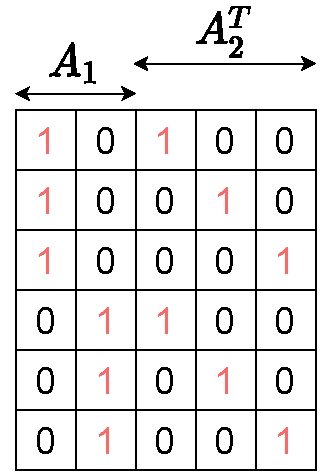
\includegraphics[height=0.25\textheight,keepaspectratio]{./Chapitre2/fig/matrix.pdf}
  \caption{An example of the matrix $A_{12}$ when $n_1=2$ and $n_2=3$.}
  \label{fig:matrix_a12}
\end{figure}
To handle the factorization constraint, first we recall the following concept.
\begin{definition}
  Given a nonnegative matrix $A$, we define its nonnegative rank by
  \begin{equation}
    \rank_{+}(A):= \min \big\{ r \geq 1: A = \sum_{i=1}^r M_i, \text{ where } \rank(M_i) = 1, M_i \geq 0, \forall i \big\}.
  \end{equation}
  By convention, zero matrix has zero (thus nonnegative) rank.
\end{definition}
So, the constraint $P = P_1 \otimes P_2$ is equivalent to $\text{mat}(P) = \vect(P_1) \vect(P_2)^T$.
By Lemma 2.1 in \citep{Joel93}, $\rank_+(A) = 1$ if and only if there exist two nonnegative vectors $u,v$ such that
$A = u v^T$. Thus, the factorization constraint is equivalent to $\rank_+\big( \text{mat}(P) \big) = 1$.

Denote $L= \text{mat}(C)$ and $M = n_1 n_2, N = n_3 n_4$. Now, Problem \eqref{factor_mmot} can be rewritten as
\begin{align}
  \min_{Q \in \bbR^{M \times N}_{\geq 0}} &\langle L, Q \rangle \\
  \text{ such that } & A_{12}^T Q 1_N = \mu_{12} \\
  &A_{34}^T Q^T 1_M = \mu_{34} \\
  &\rank_{+}(Q) = 1,
\end{align}
which is a variation of the low nonnegative rank OT problem studied in \citep{Meyer21a}.

%%%%%%%%%%%%%%%%%%%%%%%%%%%%%%%%%%%%%%%%%
\begin{proof}[Proof of \Cref{MMOT_dc_prop}]
  The inequality
  $\mmot(\mu) \leq \mmotdc_{\varepsilon}(\cT, \mu)$ follows from
  the positivity of the KL divergence. On the other hand,
  \begin{equation}
    \fmmot(\cT, \mu) =
    \inf_{P \in U_{\cT}} \langle C, P \rangle + \varepsilon \kl(P \vert P_{\# \cT}),
  \end{equation}
  because $\kl(P \vert P_{\# \cT}) = 0$, for every $P \in U_{\cT}$. As
  $U_{\cT} \subset U(\mu)$, we have
  $\mmotdc_{\varepsilon}(\cT, \mu) \leq \fmmot(\cT, \mu)$.

  Now, if $\fmmot(\cT, \mu) = 0$, then $\mmotdc_{\varepsilon}(\cT, \mu) = 0$. Conversely,
  if $\mmotdc_{\varepsilon}(\cT, \mu) = 0$, for $\varepsilon > 0$,
  then there exists $P^* \in U(\mu)$ such that $\langle C, P^* \rangle = 0$ and $P^* = P^*_{\# \cT}$.
  Thus $\langle C, P^*_{\# \cT} \rangle = 0$, which means $\fmmot(\cT, \mu) = 0$.
\end{proof}

%%%%%%%%%%%%%%%%%%%%%%%%%%%%%%%%%%%%%%%%%%%
\begin{proof}[Proof of \Cref{interpolation_prop}]
The function $\varepsilon \to \mmotdc_{\varepsilon}(\cT, \mu)$ is increasing on $\bbR_{\geq 0}$ and bounded,
thus admits a finite limit $L \leq \fmmot(\cT, \mu)$, when $\varepsilon \to \infty$, and a finite limit
$l \geq \mmot(\mu)$, when $\varepsilon \to 0$.

Let $P_{\varepsilon}$ be a solution of the problem $\mmotdc_{\varepsilon}(\cT, \mu)$.
As $U(\mu)$ is compact, when either $\varepsilon \to 0$ or $\varepsilon \to \infty$,
one can extract a converging subsequence (after reindexing)
$(P_{\varepsilon_k})_k \to \widetilde{P} \in U(\mu)$,
when either $\varepsilon_k \to 0$ or $\varepsilon_k \to \infty$.
Thus, the convergence of the marginal distributions is also guaranteed, i.e
$(P_{\varepsilon_k})_{\# \cT_m} \to \widetilde{P}_{\# \cT_m} \in U_{\cT_m}$, for every $m \in [M]$,
which implies that $P_{\varepsilon_k} - (P_{\varepsilon_k})_{\# \cT} \to \widetilde{P} - \widetilde{P}_{\# \cT}$.

When $\varepsilon \to 0$, let $P^{*}$ be a solution of the problem $\mmot(\mu)$. Then,
\begin{equation}
  \langle C, P^* \rangle \leq \langle C, P_{\varepsilon} \rangle +
  \varepsilon \kl(P_{\varepsilon} \vert (P_{\varepsilon})_{\# \cT}) \leq
  \langle C, P^* \rangle + \varepsilon \kl(P^* \vert P^*_{\# \cT}).
\end{equation}
By the sandwich theorem, when $\varepsilon \to 0$, we have
$\mmotdc_{\varepsilon}(\cT, \mu) \to \langle C, P^* \rangle = \mmot(\mu)$.
Furthermore, as
\begin{equation}
  0 \leq \langle C, P_{\varepsilon_k} \rangle - \langle C, P^* \rangle
  \leq \varepsilon_k \kl(P^* \vert P^*_{\# \cT}),
\end{equation}
when $\varepsilon_k \to 0$, it follows that $\langle C, \widetilde{P} \rangle = \langle C, P^* \rangle$.
So $\widetilde{P}$ is a solution of the problem $\mmot(\mu)$. We conclude that
any cluster point of the sequence of minimizers of $\mmotdc_{\varepsilon}(\cT, \mu)$ when
$\varepsilon \to 0$ is a minimizer of $\mmot(\mu)$. As a byproduct, since
\begin{equation}
  \kl(P^* \vert P^*_{\# \cT}) - \kl(P_{\varepsilon_k} \vert (P_{\varepsilon_k})_{\# \cT}) \geq
  \frac{\langle C, P_{\varepsilon_k} \rangle - \langle C, P^* \rangle}{\varepsilon_k} \geq 0,
\end{equation}
we also deduce that $\kl(\widetilde{P} \vert \widetilde{P}_{\# \cT}) \leq \kl(P^* \vert P^*_{\# \cT})$
(so the cluster point $\widetilde{P}$ has minimal "mutual information").

On the other hand, when $\varepsilon \to \infty$, for $\mu^{\otimes N} = \mu_1 \otimes ... \otimes \mu_N$, one has
\begin{equation}
  \langle C, \mu^{\otimes N} \rangle + \varepsilon \times 0 \geq \langle C, P_{\varepsilon} \rangle +
  \varepsilon \kl(P_{\varepsilon} \vert (P_{\varepsilon})_{\# \cT})
  \geq \varepsilon \kl(P_{\varepsilon} \vert (P_{\varepsilon})_{\# \cT}).
\end{equation}
Thus,
\begin{equation}
  0 \leq \kl(P_{\varepsilon} \vert (P_{\varepsilon})_{\# \cT}) \leq
  \frac{1}{\varepsilon} \langle C, \mu^{\otimes N} \rangle \to 0, \text{ when } \varepsilon \to \infty,
\end{equation}
which means $\kl(P_{\varepsilon} \vert (P_{\varepsilon})_{\# \cT}) \to 0$, when $\varepsilon \to \infty$. In particular,
when $\varepsilon_k \to \infty$, we have $\kl(P_{\varepsilon_k} \vert (P_{\varepsilon_k})_{\# \cT}) \to 0$. We deduce that
$\kl(\widetilde{P} \vert \widetilde{P}_{\# \cT}) = 0$, which implies $\widetilde{P} = \widetilde{P}_{\# \cT}$.

Now, as $\mmotdc_{\varepsilon}(\cT, \mu) \geq \langle C, P_{\varepsilon} \rangle$,
when $\varepsilon \to \infty$, we have $L \geq \langle C, \widetilde{P} \rangle =
\langle C, \widetilde{P}_{\# \cT} \rangle \geq \fmmot(\cT, \mu)$.
Thus $L = \langle C, \widetilde{P} \rangle = \fmmot(\cT, \mu)$, i.e.
$\mmotdc_{\varepsilon}(\cT, \mu) \to \fmmot(\cT, \mu)$ when $\varepsilon \to \infty$. In this case,
we also have that any cluster point of the sequence of minimizers of $\mmotdc_{\varepsilon}(\cT, \mu)$
is a minimizer of $\fmmot(\cT, \mu)$.
\end{proof}
%%%%%%%%%%%%%%%%%%%%%%%%%%%%%%%%%%%

% %%%%%%%%%%%%%%%%%%%%%%%%%%%%%%%%%%
% \begin{proof}[Proof of \Cref{kernel_gw_coot}]
% We write $C: = L(C_x,C_y)$, for notational convenience.
% In the setting of GW distance, we have $N=4$ and $M = 2$ with $\cT_1 = (1,2)$ and $\cT_2 = (3,4)$.
% Given a solution $P_{\varepsilon}$ of Problem \eqref{relax_mmot}, we also write
% $P_{\varepsilon, i} := (P_{\varepsilon})_{\# \cT_i}$, for short. Now,
% for any $Q_i \in U( P_{\varepsilon, i}, P_{\varepsilon, i}) \subset U(\mu)$, with $i = 1,2$.
% The optimality of $P_{\varepsilon}$ implies that
% \begin{equation}
%     \langle C, P_{\varepsilon} \rangle + \varepsilon \big[ H(P_{\varepsilon}) - H(P_{\varepsilon, 1}) -
%     H(P_{\varepsilon, 2}) \big] \leq
%     \langle C, Q_i \rangle + \varepsilon \big[ H(Q_i) - 2 H(P_{\varepsilon, i}) \big].
% \end{equation}
% Thus,
% \begin{equation}
%     2 \big( \langle C, P_{\varepsilon} \rangle + \varepsilon H(P_{\varepsilon}) \big) \leq
%     \sum_{i=1}^2 \langle C, Q_i \rangle + \varepsilon H(Q_i).
% \end{equation}
% As this is true for every $Q_i \in U(P_{\varepsilon, i}, P_{\varepsilon, i})$, we have
% \begin{equation}
%     \begin{split}
%         \frac{1}{2} \sum_{i=1}^2
%         \text{OT}_{\varepsilon}(P_{\varepsilon, i}, P_{\varepsilon, i})
%         &= \frac{1}{2} \sum_{i=1}^2 \inf_{Q_i \in U(P_{\varepsilon, i}, P_{\varepsilon, i})}
%         \langle C, Q_i \rangle + \varepsilon H(Q_i) \\
%         &\geq \langle C, P_{\varepsilon} \rangle + \varepsilon H(P_{\varepsilon}) \\
%         &\geq \inf_{P \in U(P_{\varepsilon, 1}, P_{\varepsilon, 2})}
%         \langle C, P \rangle + \varepsilon H(P) \\
%         &= \text{OT}_{\varepsilon}(P_{\varepsilon, 1}, P_{\varepsilon, 2}).
%     \end{split}
% \end{equation}
% The second inequality holds because $P_{\varepsilon} \in U(P_{\varepsilon, 1}, P_{\varepsilon, 2})$. Thus,
% \begin{equation} \label{sinkhorn_div}
%   \text{OT}_{\varepsilon}(P_{\varepsilon, 1}, P_{\varepsilon, 2}) -
%   \frac{1}{2} \sum_{i=1}^2 \text{OT}_{\varepsilon}(P_{\varepsilon, i}, P_{\varepsilon, i}) \leq 0.
% \end{equation}
% The left-hand side of the inequality \eqref{sinkhorn_div} is nothing but the Sinkhorn divergence between $P_{\varepsilon, 1}$ and
% $P_{\varepsilon, 2}$ \citep{Ramdas17}. As the kernel $C$ is conditionally negative definite if and only if for every
% $\varepsilon > 0$, the kernel $e^{-C / \varepsilon}$ is positive definite \citep{Schoenberg38}, by Proposition 5 in \citep{Janati20},
% the inequality in \ref{sinkhorn_div} becomes an equality. As a consequence, for $i=1,2$, if
% $Q_{\varepsilon, i} \in U( P_{\varepsilon, i}, P_{\varepsilon, i})$ is the (unique) optimal plan of the entropic OT problem
% $\text{OT}_{\varepsilon}(P_{\varepsilon, i}, P_{\varepsilon, i})$, then we must have
% \begin{equation}
%   \langle C, P_{\varepsilon} \rangle + \varepsilon \big[ H(P_{\varepsilon}) - H(P_{\varepsilon, 1}) -
%   H(P_{\varepsilon, 2}) \big] =
%   \langle C, Q_{\varepsilon, i} \rangle + \varepsilon \big[ H(Q_{\varepsilon, i}) - 2 H(P_{\varepsilon, i}) \big],
% \end{equation}
% or equivalently, $Q_{\varepsilon, 1}$ and $Q_{\varepsilon, 2}$ are also solutions of Problem \eqref{relax_mmot}.

% Now, by \Cref{interpolation_prop}, when $\varepsilon \to \infty$, a cluster point
% $P^* = P^*_{\# \cT_1} \otimes P^*_{\# \cT_2}$ of the sequence of minimizers $(P_{\varepsilon})_{\varepsilon}$ induces a solution
% $(P^*_{\# \cT_1}, P^*_{\# \cT_2})$ of the COOT problem. In particular, $P^*_{\# \cT_i}$ is a cluster point of
% $(P_{\varepsilon, i})_{\varepsilon}$ and there exists a cluster point $Q^*_i$ of
% $(Q_{\varepsilon, i})_{\varepsilon}$ in $U(P^*_{\# \cT_i}, P^*_{\# \cT_i})$, for $i=1,2$. But still by
% \Cref{interpolation_prop}, we also have that $Q^*_i = (Q^*_i)_{\# \cT_1} \otimes (Q^*_i)_{\# \cT_2}$. Thus,
% $Q^*_i = P^*_{\# \cT_i} \otimes P^*_{\# \cT_i}$
% and the solution $(P^*_{\# \cT_1}, P^*_{\# \cT_2})$ of the COOT problem satisfies:
% $\langle C, P^*_{\# \cT_1} \otimes P^*_{\# \cT_2} \rangle =
% \langle C, P^*_{\# \cT_1} \otimes P^*_{\# \cT_1} \rangle =
% \langle C, P^*_{\# \cT_2} \otimes P^*_{\# \cT_2} \rangle$. The equality between GW distance and COOT then follows,
% and $P^*_{\# \cT_1}$ and $P^*_{\# \cT_2}$ are two solutions of the GW problem.

% If furthermore, the kernel $C$ induces a strictly positive definite kernel, then by Proposition 5 in \citep{Janati20},
% we deduce that $P_{\varepsilon, 1} = P_{\varepsilon, 2}$. One can also use the following reasoning:
% in the finite setting, a strictly positive definite kernel is necessarily universal (see for example Section 2.3 in
% \citep{Borgwardt06}), and the kernel $C$ defined on $(X \times Y)^2$ is necessarily a (symmetric)
% Lipschitz function with respect to both inputs. So, the Sinkhorn divergence vanishes if and only if
% $P_{\varepsilon, 1} = P_{\varepsilon, 2}$ \citep{Feydy19}. From either reasoning, we conclude that
% $P^*_{\# \cT_1} = P^*_{\# \cT_2}$.
% \end{proof}